\documentclass[../main.tex]{subfiles}
\graphicspath{{\subfix{../images/}}}
\begin{document}
	
	\chapter{The CCD characterization procedure}
		\section{Developing the characterization procedure}
		The CCD characterization procedure will be developed in this chapter. It covers the metrics outlined in the preceding chapter. The initial thoughts and considerations will be described first, and will serve to illustrate the design process. The results from preliminary tests are described. From these, the conclusions that lead to the final measurement plan will then be presented. The characterization procedure will be presented as a measurement plan. Lastly, the results will be summarized, and the calibration procedure is described.
		
		\subsection{The initial experimental setup for test plan development}\label{sec:setup}
		The camera described in table \ref{table:testcam} was used in the development of this characterization procedure. The experimental setup is seen in figure \ref{fig:setup}. 
		
		\begin{figure}
			\centering
			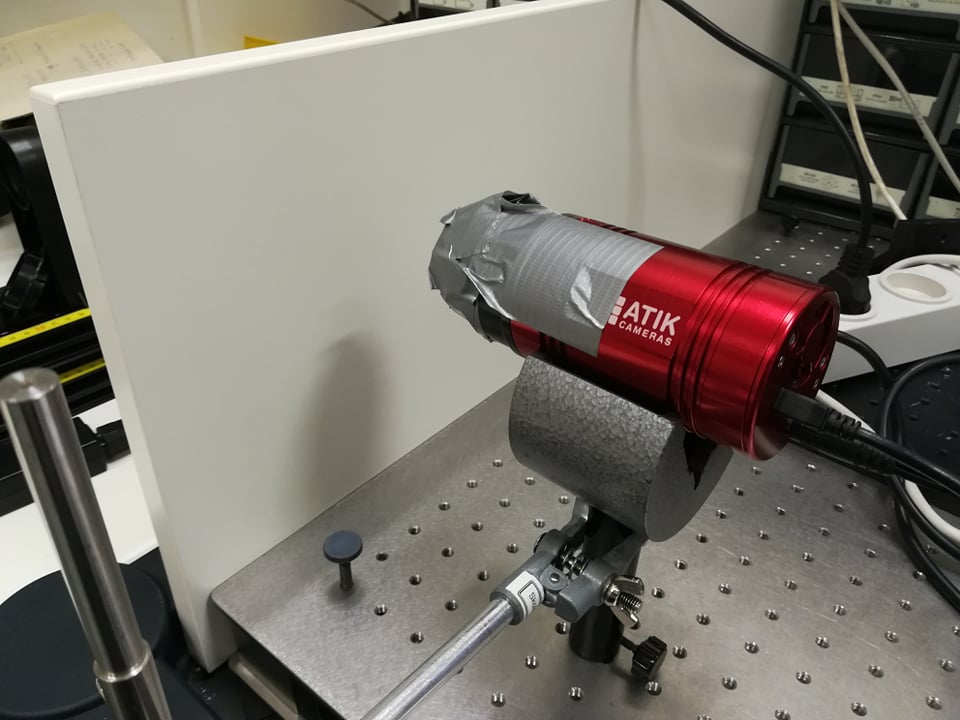
\includegraphics[width=0.99\textwidth]{setup.jpg}
			\caption{The experimental setup used both for light and dark frame acquisitions. The setup consists of the Atik 414EX detector resting on a stand. A pinhole is attached to the detector. The pinhole is constructed from a hole made with a needle in a piece of thick black cardboard. The detector is pointed into a white lacquered wooden screen, and is connected via USB2 to a lab computer. The setup is placed in a dark-room. This is to ensure we can acquire a proper dark frames when the light is turned off in the room.}
			\label{fig:setup}
		\end{figure}
		
		The setup consists of the camera resting on a stand, pointed into a white lacquered wooden screen. The camera is connected via USB2 to the lab computer. Since the setup for dark frames requires a sufficiently dark room, an in-house darkroom is used. The equipment used, perhaps save for the detector it self, is readily found in most university school labs.
		For all exposures for which the camera is exposed to light (hereafter referred to as \textbf{light frames}), the ambient room lighting was used. The ambient light is a double fluorescent bulb, and the light can be dimmed to roughly half of the flux by turning off half the bulbs. Since the Atik 414EX detector does not have a shutter, rapid saturation was seen for very small exposure times, in a lit room environment. To circumvent this issue, a pinhole was constructed from heavy black cardboard and mounted with tape. The cardboard was poked with a small needle to create a small hole. This pinhole also serves to focus the light, and create an image at the detector plane.
		For all dark frames, the same configuration was used, but with ambient light and computer screens turned off. 
		
		\begin{table}[]
			\centering
			\begin{tabular}{|c|c|}
				\hline
				\textbf{Model name }& Atik 414EX mono \\
				\textbf{Chip name}& Sony ICX 825\\
				\textbf{Readout noise (typical)}& 5$e^-$\\
				\textbf{Gain factor}& 0.28$e^-$/ADU\\
				\textbf{Cooling $\Delta T$}& $-30^\circ$\\
				\textbf{Dark current}& $\sim 0.001 e^- / s\;$ at $\;-10^\circ$ \\
				\textbf{ADC}& 16 bit\\
				\textbf{Pixel size}& $6.45 \mu m \times 6.45 \mu m$\\ 
				\textbf{Shutter}&No\\
				\hline
			\end{tabular}
		\caption{Relevant data specs for the \textbf{Atik 414EX mono} camera \cite{atik414specs}}\label{table:testcam}
		\end{table}
			
	\subsection{Preliminary thoughts and considerations}
	The starting point for developing an experimental procedure are the initial thoughts and considerations about how to best measure the various metrics. From that, iteratively, the final procedure will be developed. 
	
	\subsubsection{Acquiring data and reducing noise}
	Here, practical noise reduction steps that should be applied during acquisition, will be described. 
	
	For any measurement, we should take steps to reduce the noise in the image. Dark current can be reduced by cooling the chip before acquiring data frames. Readout noise is \textbf{Gaussian} and the signal to noise ratio is reduced by a factor of $1/\sqrt{N}$ for $N$ measurements. For each datapoint, before computing the desired variable, like dark current for a specific temperature, we should, at that temperature, acquire $N$ frames, and construct a mean image from these $N$ frames. Typically $N$ is chosen to be as large as is practically feasible. The value of the experimental metric is then computed from that average frame. 
	
	Initially, $N = 100$ was chosen to achieve a high degree of noise reduction. It was seen that due to general low noise levels in the detector in the cooled setting (see next section), a value of $N = 10$ was sufficient. The temperature was chosen to be $T = -10^\circ$ C, due to reasons outlined in the next section.
	
	\begin{figure}[h!]
		\centering
		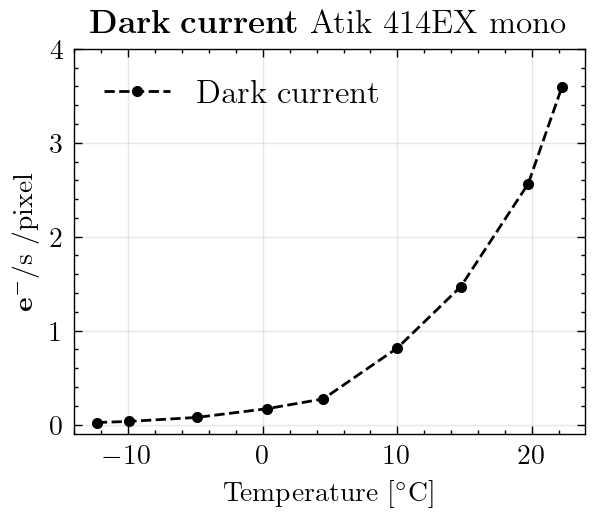
\includegraphics[width=0.6\textwidth]{darkcurrent_versus_temperature_preliminary.png}
		\caption{Preliminary dark current measurement, performed at the office in sub-optimal settings, to get a first glimpse of the behavior of this variable.}
		\label{fig:dcprelim}
	\end{figure}
		\subsubsection{Background noise and dark current}
		A preliminary investigation of the noise levels of the chip was carried out at a desktop in an office A very primitive experimental setup was used. This short experiment confirms that dark current is strongly dependent on temperature. See figure \ref{fig:dcprelim}. Since the camera cooler can cool to a temperature gradient of $\Delta T = 30 ^\circ $C, the temperature $T = -10 ^\circ$ C was chosen. Since the cooling system works as a temperature gradient, it is not feasible to go much lower. These steps ensure that we can minimize dark current and read-out noise.
		
		\subsubsection{Master bias and flat field frames}
		Bias images are frames with the smallest possible exposure time. This exposure time is $0.001s$ for the Atik 414EX detector. For the construction of the master bias frame, we choose $N = 300$. This is rather arbitrary, but easily achieved at this short an exposure time. The bias frames are acquired in a dark setting with no light. This frame should be subtracted from all other data points. The same repeat number is chosen for the master flat-field frame, where the exposure time was chosen to be $10s$.  The flat-field frames are acquired in a lit room setting. 
		
		For both the bias frames and the flat-field frames, as chosen above $T= -10^\circ$. This is to reduce dark current.
		
		\begin{figure}[h!]
			\centering
			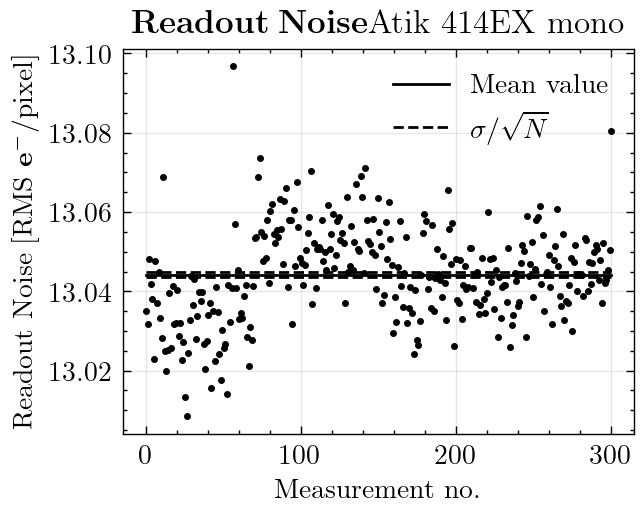
\includegraphics[width=0.65\textwidth]{readout_noise_measurement_atikcam.png}
			\caption{A plot of the measured readout noise level as a function of repeat number, along with the found mean value (plotted as a solid line) and relative error of the measurement of the mean value (plotted with dashed lines). The mean value is tabulated with its relative error in table \ref{table:results}. Here the temperature is kept constant by setting the camera cooler to $-10^\circ$. The cooler exhibits small fluctuations over time around the temperature setpoint. The systematic variations observed in this figure is likely due to small fluctuations in the temperature, as readout noise is dependent on temperature (see figure \ref{fig:readoutnoise}).}
			\label{fig:ronmeas}
		\end{figure}
		
		\subsubsection{Readout noise level}
		We need to compute the readout noise level of the camera, at the temperature at which it will be operated. This is to estimate the proper gain factor to be used in the characterization procedure following equation (\ref{eq:gainfactorest}). The series of bias frames acquired in the construction of the master bias frame may be used to compute the readout noise as described in section \ref{ron}. This yields the readout noise level in ADU. The measurement of this readout noise level is plotted, as a function of repeat number in figure \ref{fig:ronmeas}, along with the mean value, also tabulated in table \ref{table:results} and corresponding relative error in the measurement.
		\begin{figure}[h!]
			\centering
			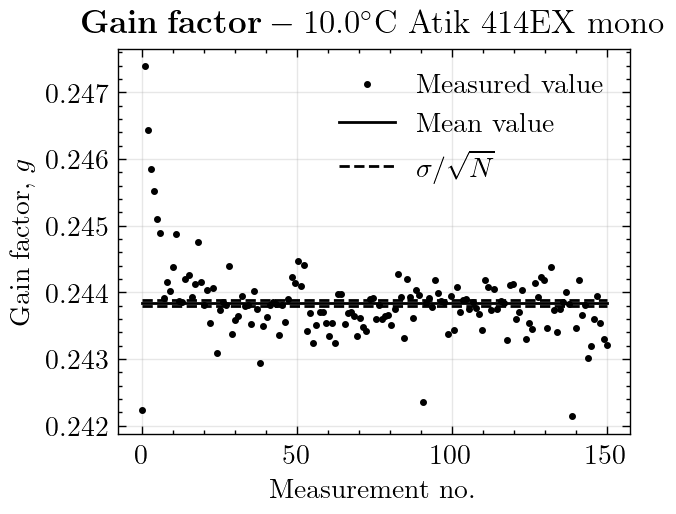
\includegraphics[width=0.65\textwidth]{gain_factor_measurement_atikcam.png}
			\caption{Measurements of the gain factor, using equation (\ref{eq:gainfactorest}) with $N=150$ repeats ($300$ flat-field frames, since we need two unique frames for each gain factor computation). The mean value is tabulated with the error in table \ref{table:results} and shown here as a black filled line. The relative error is plotted with dashed lines around the mean value. Here we observe that the first few data points lie significantly higher than the remaining. As with the readout noise estimation in figure \ref{fig:ronmeas}, this may be due to the cooler settling at the desired temperature. Gain is expected to be temperature-dependent, as is also evident in figure \ref{fig:gainvtemp}. These data points should be excluded, and for future reference, the cooler should be allowed time to settle properly before measurement acquisition begins.} 
			\label{fig:gainmeasurement}
		\end{figure}
		
		\subsubsection{Gain factor}
		The gain factor may be calculated by using two subsequently acquired flat-field frames from the data series acquired in the construction of the master flat-field frame. Following equation (\ref{eq:gainfactorest}) and using the calculated readout noise in ADU yields a gain factor. The error in the measurement of this gain factor can be reduced by repeating this calculation for several pairs of flat fields from the data series. The measurement of the gain factor, using $N = 150$ repeats ($300$ flat-field frames, since we need two unique frames for each gain factor computation), may be seen in figure \ref{fig:gainmeasurement}, where the mean value and error has been plotted. Gain is also expected to exhibit a temperature dependence. To make sure that the temperature dependence that is observed in the measurement of the readout noise (see figure \ref{fig:readoutnoise}), is true, and not due to temperature dependence in the gain factor, we should measure the gain factor as a function of temperature. This may be seen in figure \ref{fig:gainvtemp}.
	
		\begin{figure}[h!]
			\centering
			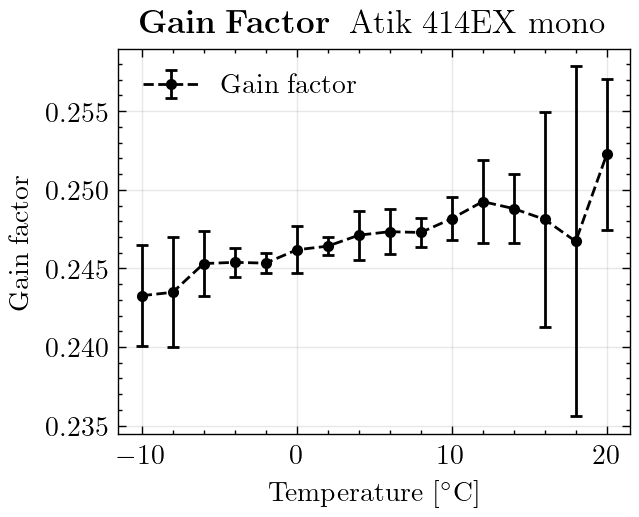
\includegraphics[width=0.65\textwidth]{gain_versus_temperature_atikcam.png}
			\caption{Gain factor measured according to equation (\ref{eq:gainfactorest}), as a function of temperature. A weak temperature correlation is observed. It is unclear to the author, why the first two and latter three points exhibit a greater uncertainty, but it may be due to the stability of the detector cooling component.}
			\label{fig:gainvtemp}
		\end{figure}
		
		\subsubsection{Exposure times for linearity}\label{sec:explin}
		The linearity measurement consists of acquiring exposures of the white screen. This is done as a function of exposure time, to study the linearity of the response in measured photons. We should first determine which exposure time interval to use. At first, a 100s exposure is acquired with all light in the room turned on. In that frame considerable saturation was observed. It was thus concluded that an exposure time of 100 seconds was a good data point for the last acquisition. 
		\begin{figure}[h!]
			\centering			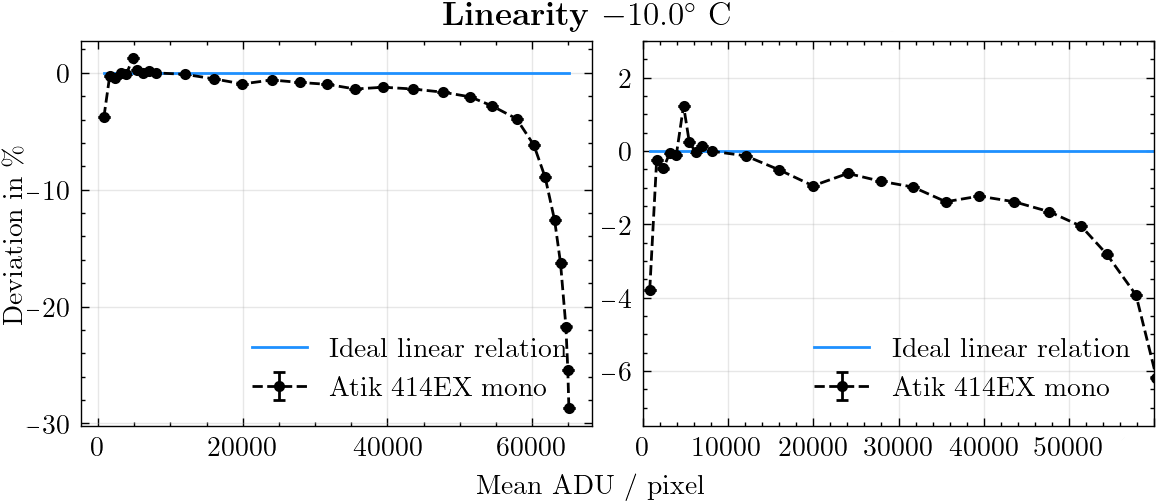
\includegraphics[width=0.999\textwidth]{linearity_notimecorrect_final.png}
			\caption{Left: A plot of the percentage deviation from ideal linearity computed according to equation  \ref{eq:fluxcorrect_timecal} for each exposure time after meaning across $N$ frames. A significant deviation is observed for the first data point, the $1s$ exposure. This is likely due to issues with the time keeping of the detector, and necessitates a time calibration as described below. The sixth datapoint lies significantly above the remaining, and subsequent measurements should determine if this is a true feature of the linearity curve, or a systematic error. It is not present in figure \ref{fig:linearitydim}, so the latter explanation is most likely the correct one. Right: A zoom of the left pane.}
			\label{fig:linearity}
		\end{figure}
		
		The choice of exposure times generally relies on trial and error, to decide what range of exposure times we should use, at a given light source intensity. At first frames at exposures between $0.001s$ and $10s$ in $1s$, between $10s$ and $100$s in $10s$ intervals, and $100s$ and $110s$ in $1s$ intervals were acquired. It was found that the light source stability varies slightly, resulting in greater uncertainty in short exposure measurements, and hence it was chosen to omit $0.001$ seconds, and instead acquire frames in the interval $1s$ to $10s$ in 1-second intervals, in addition to the data sequence described just above. In the interval $10s$ to $110s$, data points were acquired in $5s$ intervals.  
		
		Measurements with exposure times shorter than $10s$ are found to be more uncertain. These are the first 10 data points in figure \ref{fig:linearity}. This is likely due to a time offset resulting from the lack of shutter on the testing camera. In addition to the time calibration in question, described below, it is recommended that a dimmer light source be used, and instead, frames are acquired at longer exposure times that pose lesser uncertainty in the measurements. This ensures we can decouple the low-ADU regime from the short exposure time regime.
		\begin{figure}[h!]
			\centering			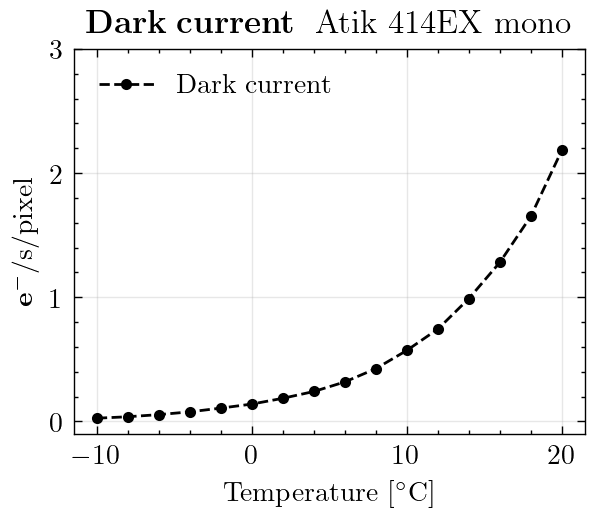
\includegraphics[width=0.6\textwidth]{darkcurrent_versus_temperature.png}
			\caption{A plot of dark current as a function of temperature. The data points are computed by acquiring 100 dark frames at an exposure time of $10$s, at each temperature. Dark current is computed according to equation \ref{darkcurrenteq}. }
			\label{fig:darkcurrent}
		\end{figure}
		\subsubsection{Noise as a function of temperature}
		Readout noise and dark current are expected to be temperature-dependent. Hence, in the entire cooling range of the camera,  dark frames were acquired to study the behavior of these physical effects. Exposure times are chosen such that the minimal exposure time is chosen for the readout noise images. Dark current is time-dependent, and should be negligible in this regime. For dark current frames, it is crucial to pick an exposure time such that the dark current contribution is greater (by a considerable amount, higher orders of magnitude) than the readout noise contribution. Dark current follows a \textbf{Poissonian} distribution, and to recover this underlying distribution, longer exposure times are chosen. Since this requires \textbf{very} long times of exposure, it is more practical to pick an exposure time of $10s$, and then mean over $N = 100$ acquired images at this temperature, to reduce the noise contribution.
	\begin{figure}[h!]
		\centering			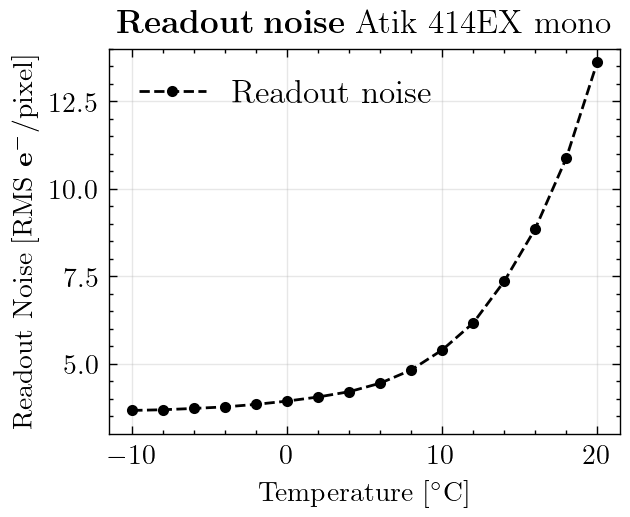
\includegraphics[width=0.6\textwidth]{readoutnoise_versus_temperature.png}
		\caption{A plot of readout noise as a function of temperature, using a gain factor dependent on temperature from figure \ref{fig:gainvtemp}. The datapoints have been constructed by acquiring 100 dark frames at an exposure time of $0.001$s at each temperature. Readout noise is computed according to section \ref{sec:rondc}. The temperature dependence observed is due to thermal fluctuation in the electronics introducing extra electrons. }
		\label{fig:readoutnoise}
	\end{figure}
		
		\subsubsection{Hot pixel treatment}\label{sect:hotpix}
		It is crucial to treat hot pixels. One way to do this is to realize that hot pixels are those in which dark current does not exhibit a linear temporal behavior. Acquiring a \textit{very} long exposure, here chosen as a $1000s$ exposure, and a medium-long (considerably shorter than the former) exposure, here chosen to be a $90s$ exposure, we can study the dark current in each pixel, and determine if there is a linear relationship between the two frames.
		\begin{figure}
			\centering			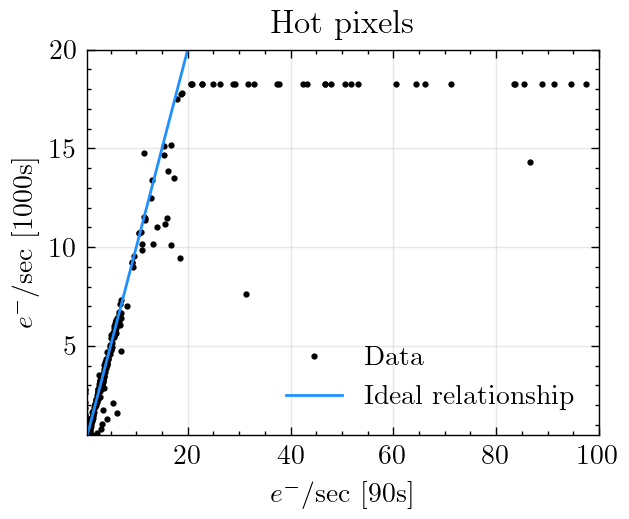
\includegraphics[width=0.7\textwidth]{hot_pixels_test.png}
			\caption{Two exposures acquired at exposure times of respectively $90s$ (first axis) and $1000s$ (second axis). The flattened arrays of data (pixel values of dark current) are sorted, and values of dark current above the threshold described in section \ref{sect:hotpix} are plotted. Outside the range of a linear relationship between the two exposures, pixels are considered hot. This is usually above some value of the dark current, here qualitatively judged to be at $7.5 e^-/\text{sec}$. This value is chosen as the cutoff. Any pixel that displays a dark current above this value is defined as a hot pixel, and its index is used to define a mask. This mask can be seen in figure \ref{fig:hotpixmask}. The flattening of the curve at the top is due to saturation of the pixels. 
			}
			\label{fig:hotpix}
		\end{figure}
		
		Small values of the dark current are most accurately measured in the long exposure image, while the short exposure image will allow for the large dark current values to be accurately measured. We can note that for the Atik 414EX detector, readout noise at $T = -10^\circ$C, is around $3$-$4$ electrons per image. Dividing that by the exposure time in the short exposure image, $90s$, corresponds to a dark current of about $0.33-0.44 e^-/\text{sec}$. The dark current contribution should be significantly greater than the readout noise level, to identify the Poissonian distribution of the thermal noise. Thus we may conclude that the smallest measurable dark current in that image will be around twice that \cite{CCDdatareductionguide}. This treatment can be seen in figure \ref{fig:hotpix}. For this analysis applied to the Atik 414EX detector, a value of $7.5 e^-/\text{sec}$ was chosen as the cutoff for the definition of a hot pixel. We use this value as a filter, below which we do not include the pixel in the following treatment. Such a mask can be seen in figure \ref{fig:hotpixmask}. $94$ hot pixels were identified applying this analysis on the Atik 414EX detector.
		
		\begin{figure}
			\centering			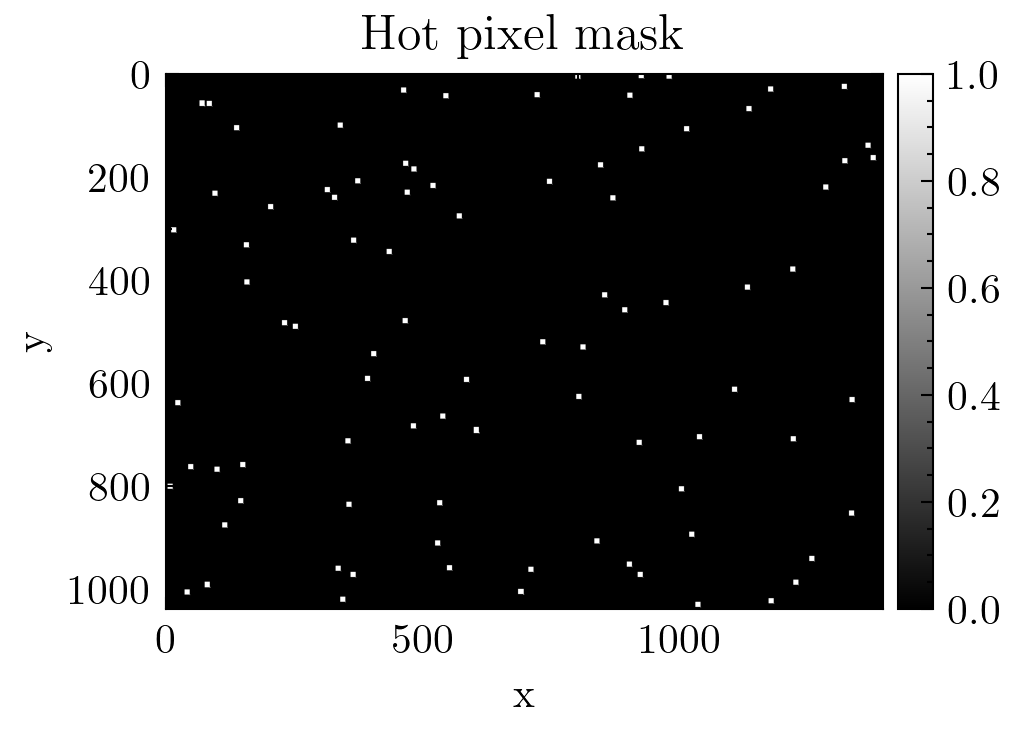
\includegraphics[width=0.95\textwidth]{hot_pixel_mask.png}
			\caption{The hot pixel mask. For the Atik 414EX detector, a value of $7.5 e^-/\text{sec}$ was chosen as the cutoff. White spots mark the pixels that should be omitted in the other analyses. Here the white spots have been enlarged to illuminate the concept. $94$ hot pixels were identified by applying this analysis on the Atik 414EX detector.}
			\label{fig:hotpixmask}
		\end{figure}
		
		We scatter plot the pixels in the short exposure against the same pixels in the long exposure. The range within which the data points seem to follow a linear relationship is judged qualitatively. The remainder are considered hot, and a mask is constructed. For the Atik 414EX detector, this value is around a dark current of $7.5 e^-/$sec. These pixels are then marked, and an image mask is produced. This mask marks which pixels to omit in the other analysis.
		
		\subsubsection{Testing of initial assumptions}
		In our experimental setup, assumptions are made that must be tested. The two most important ones are that 
		\begin{itemize}
			\item The camera has a well-calibrated temporal zero-point. This means a 10-second exposure is physically the frame resulting from light being able to enter the chip for exactly 10 seconds. This is of particular importance since the camera used for the development of the testing procedure does not have a shutter.
			\item The light source used is stable during exposure, so we can accurately compare ADU intensities between different frames. The ambient room light is used, which consists of double fluorescent light bulbs. We should as a null hypothesis expect to find fluctuations, and potentially even drifts in the light source over time.
		\end{itemize}
		The latter assumption can be tested by analyzing the many exposures taken during the first linearity sequence. We may plot the percentage deviation from the mean ADU (mean across all $N=100$ exposures at a given exposure time) as a function of exposure time. Both of these tests are described in detail in the following two sections. 
		
		\subsection{Stability of the lightsource}\label{sec:stabillitylight}
		Testing whether the light source flux is stable over time, is achieved via preliminary investigations utillizing the wealth of data acquired during the linearity measurement sequence. At each exposure time, $N = 100$ repeat frames were recorded. From each repeat series, a mean image is constructed. The mean ADU/pixel in this image is our reference value. The percentage deviation in the mean ADU/pixel, in each of the individual repeat frames of the sequence, is then plotted as a function of time. This makes it possible to qualitatively judge the stability of the light source as a function of time. Such a plot can be seen in figures \ref{fig:lightsourcestability1to10},  \ref{fig:lightsourcestability20to100},  \ref{fig:lightsourcestability101to110}.
		
		All of the exposures in the $1s$ to $10s$ range show fluctuations within half a percent, with $1s$ and $10s$ as exceptions. $1s$ is the orange line that starts at a deviation of around $1\%$, dips to around $-1.5\%$ at repeat no. 25, and slowly rises. These sudden changes can likely be explained by electricity being used elsewhere in the building. The $10s$ exposure is the light blue that slowly dips from $-0.5\%$ to $0.5\%$. For longer exposure, in the range $20s$ up to $110s$ the light source remains in general \textit{very} stable. This is due to the statistical nature of the measurement. For longer measurements, a transient flux change is of lesser importance.
		
		Measurement acquisition schemes to eliminate this variability in the flux will be presented below. 
		
		\begin{figure}
			\centering			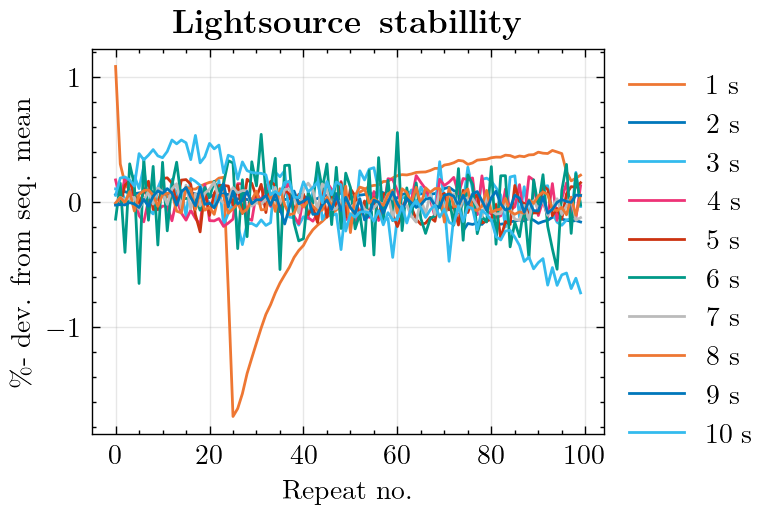
\includegraphics[width=0.8\textwidth]{lightsource_1to10.png}
			\caption{A plot of the temporal dependence in the light source intensity (flux) across exposure times $1s, 2s \dots 10s$. All show fluctuations within half a percent. Here the $1s$ and $10s$ exposures series are exceptions. $1s$ is the orange line that starts at a deviation of around $1\%$, dips to around $-1.5\%$ at repeat no. 25, and slowly rises. The $10s$ exposure is the light blue that slowly dips from $0.5\%$ to $-0.5\%$. These sudden changes can likely be explained by electricity being used elsewhere in the building. In addition, during a $1s$ exposure, any drifts or changes to the flux that are sudden and last for a short amount of time will easily influence the mean value, while it will be of less importance during longer exposures. This also explains why the order of magnitude of the deviations seen here are greater than those of figures \ref{fig:lightsourcestability20to100} and \ref{fig:lightsourcestability101to110}. Drifts, such as the one seen for the $1s$ exposure after repeat no. 25, and the $10s$ exposure, may be due to power usage in the building changing over time. }
			\label{fig:lightsourcestability1to10}
		\end{figure}
		\begin{figure}
			\centering			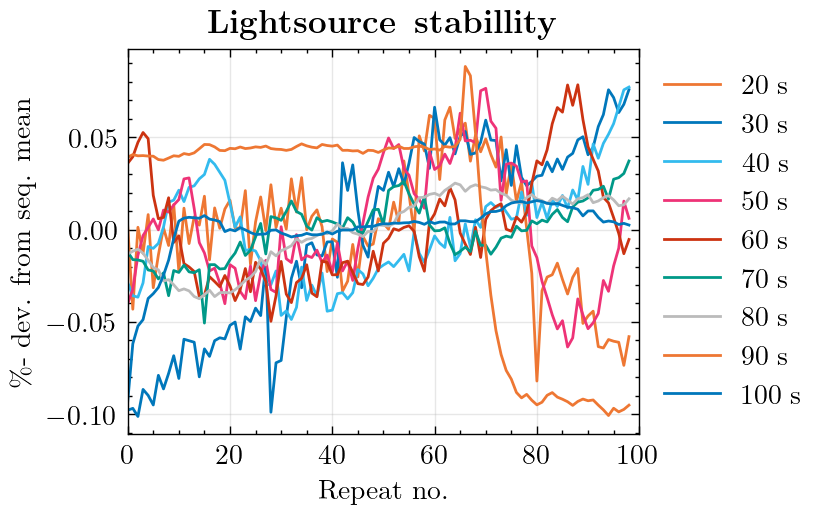
\includegraphics[width=0.8\textwidth]{lightsource_20to100.png}
			\caption{A plot of the temporal dependence in the lightsource intensity (flux) across exposure times $20s, 30s \dots 100s$. Here all intensities remain stable to a \textit{small} percentage deviation. A sudden dip is seen in the (with orange) $90s$ exposure. The (relative to shorter exposures) small deviations in the intensity of the light, may here be explained statistically, as many photons are acquired during a long exposure, and small drifts and sudden jumps in the intensities will be of lesser importance. As with figure \ref{fig:lightsourcestability1to10}, we observe both sudden dips and drifts over time in the intensity, that are likely occurring due to the same reasons.}
			\label{fig:lightsourcestability20to100}
		\end{figure}
		\begin{figure}
			\centering			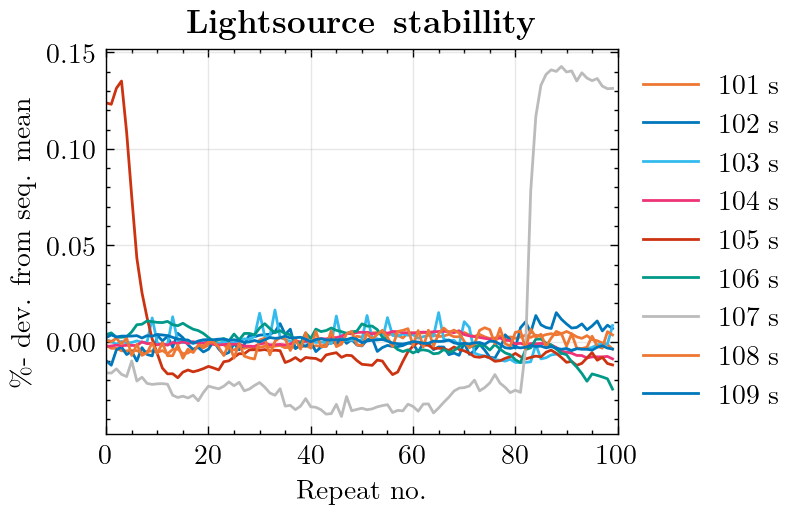
\includegraphics[width=0.8\textwidth]{lightsource_101to110.png}
			\caption{A plot of the temporal dependence in the lightsource intensity (flux) across exposure times $101s, 102s \dots 110s$. Here all intensities remain stable to a \textit{very small} percentage deviation, again likely due to the long exposure times. Jumps are seen in the $105s$ and $107s$ series.  }
			\label{fig:lightsourcestability101to110}
		\end{figure}
		
		The plotted deviations cannot be used as a correction, since this does not include the correlation of instability between exposure times. Instead, it is proposed that a reference exposure be utilized. Within a given repeat sequence, one may use a reference of, say, a $10s$ exposure by alternating between the chosen \textbf{reference exposure}, and the \textbf{desired exposure time}. Thus we acquire an exposure data series like $[10s, 1s, 10s, 1s, 10s, \dots 10s, 2s, 10s, 2s,\dots]$, making sure we cover the entire range of exposure times. For each frame in the series, we then have a 10-second exposure just before and right after. For the Atik 414EX detector, the software designed for the camera only enables the user to set up a sequence of 10 data points to be acquired automatically but allows that sequence to be repeated. Hence it was most practical for the analysis to acquire data in the series $[10s, 1s, 10s, 2s, 10s, 3s, 10s, \dots 10s, 9s, 10s]$, repeat that N times, and then repeat until the desired exposure time range has been covered. $N=10$ repeats was chosen since this was sufficient to reduce noise levels for that detector. The two reference measurements to use in the correction of a given frame will then be the two taken at adjacent times. 
		
		The flux of the light source at the time of our desired frame then lies somewhere in between, assuming a linear change between the acquisition of the two reference frames. These assumptions of local monotonicity of the light source flux are justified by considering figures \ref{fig:lightsourcestability1to10},  \ref{fig:lightsourcestability20to100},  \ref{fig:lightsourcestability101to110}. 
		
		In this way we are also able to correct for the potential long temporal drift of the intensity. Let $\bm F(x[s]) = \text{mean}\left(\text{Image}([s])\right)$ be interpreted as the mean flux (the mean ADU value) in an image of exposure time $s$ in seconds. We may correct for the instability, using a 10 second reference exposure, for a given frame via the computation
		\begin{equation}\label{eq:fluxcorrect_notimecal}
			\bm F(x [s])_\text{corrected} = \frac{\bm F(x [s])}{\frac12\left[\bm F(10s)_\text{before}+\bm F(10s)_\text{after}\right]} * \frac{10s}{x[s]},
		\end{equation}
		where the last factor of 10s, divided by the exposure time, is to account for the relation between the 10 seconds and actual exposure times, in the ideal case where there is no time offset.
	\begin{figure}[h!]
	\centering			
	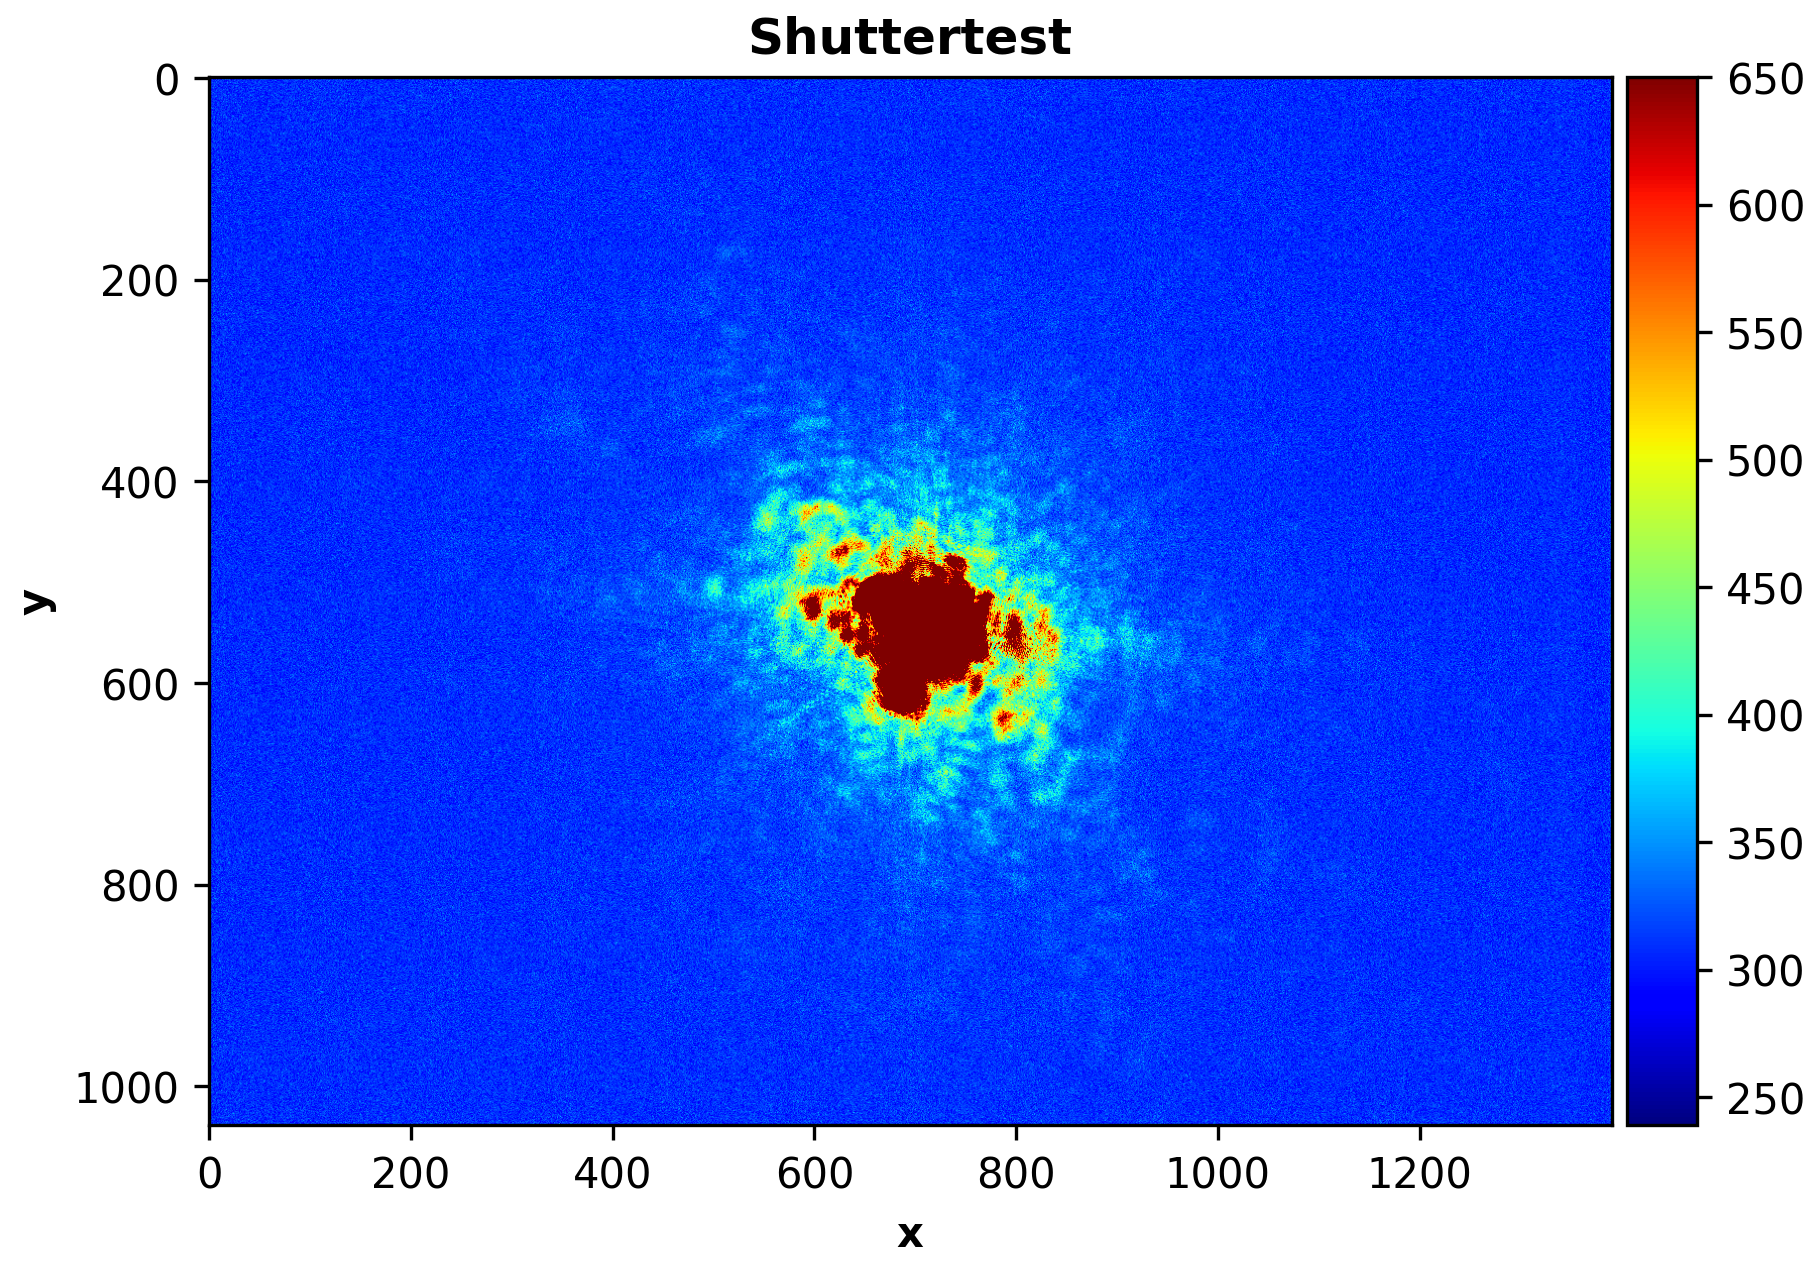
\includegraphics[width=0.8\textwidth]{shutter_test.png}
	\caption{An image of the white screen, taken in a dark room setting, shining a red laser onto the screen. If the lack of a shutter introduces a significant effect, we should expect to see smear in the image. None is seen. }
	\label{fig:shuttertest}
	\end{figure}
	\subsection{Time calibration}\label{sec:timecal}
	The next assumption we must test is the time keeping ability of the detector.
	If the detector in question is not shielded from incoming photons during readout of the pixels, artifacts such as smear may occur in the image. The exposure time will be longer. The Atik 414EX detector does not have a mechanical shutter, and the readout time is tabulated as $1/15s$ in the specifications. For a $1s$ exposure time, this corresponds to an error of $\sim 6.6\%$, which introduces a significant deviation. A time calibration should be performed to estimate this offset. This time offset should be added to the exposure time. 
	
	First we may investigate the importance of the lack of shutter in the test procedure camera. By choosing a strong focused light source, such as a laser, if the chip is exposed during readout, we should see some degree of smear in the image. The result of this simple test can be seen in figure \ref{fig:shuttertest}. We do not observe smear, indicating that any time offset is expected to be small.
	
	A series of measurements were acquired to study if the zero-point of time keeping was actually $0s$. A preliminary estimate is obtained by acquiring eight frames. Note that, under the assumption that our detector is linear, for a given frame $\textbf{Image(}\text{Exposure time}\textbf{)}$, we must expect for a perfect time calibration that 
	
	\begin{equation}
		\frac{\text{Image}(21s) - \text{Image}(1s)}{\text{Image}(11s) - \text{Image}(1s)} = \frac{\text{Image}(20s) - \text{Bias}}{\text{Image}(10s) - \text{Bias}}
	\end{equation}
	Or that 
	\begin{equation}
		\frac{\textbf{mean}(\text{Image}(21s) - \text{Image}(1s))}{\textbf{mean}(\text{Image}(11s) - \text{Image}(1s))} - \frac{\textbf{mean}(\text{Image}(20s) - \text{Bias})}{\textbf{mean}(\text{Image}(10s) - \text{Bias})} = 0,
	\end{equation}
	where \textbf{mean}$()$ refers to the mean ADU/pixel within an image. The result of this, for the Atik 414EX detector, being $0.0063$ indicates a time offset which must be determined properly, and applied as a correction. 
	
	It has now been determined that an exposure time of $1s$ should be correctly interpreted as an exposure time of $1s + \Delta t$. $\Delta t$ should be deduced experimentally. Via a separate linearity measurement series using more datapoints, in the uncertain interval of $1s - 10s$ we can get the first estimate of $\Delta t$ by fitting a linear function to the data points and determining the roots of polynomial. This exposure time interval was chosen since the readout time will significantly impact exposure times in this regime.
	
	If there is a time offset, the line will intersect the first axis at a point different from the origin. The intersection point on the first axis should be subtracted. For a negative value of the intersecting point on the first axis, a subtraction physically corresponds to a longer exposure time. Deviations from the initial linear fit may be seen in figure \ref{fig:timecaldev}, once again indicating that shorter exposure times are more uncertain. 

	Since we still observe fluctuations in the low exposure regime, we may try to circumvent the issue of fluctuations by using $1s$ exposure frames as a reference, and acquiring one $2s$ frame, "sandwiched" (in time) by two reference measurements of $1s$ exposure. Let us define $\bm F_A, \bm F_B$ to be the flux of the $1s$ reference frames that are taken before and after the $2s$ frame, respectively. Correspondingly $\bm F_2$ is the flux of the $2s$ frame. By flux we understand the mean value in the image, after bias frame subtraction, and hot pixel and flat field corrections have been applied. The corrections are important in this calibration procedure, since they correct for a shift in the mean flux. This will influence the ratio of fluxes considered next.
	
	The relation between the mean value of the flux before and after, to the flux of the $2s$ frame, should be equal to the relation between the \textit{true} exposure times. The ratio should be divided by $2$ to correct for the double exposure time.
	\begin{align}\label{eq:timecorrectionfactor}
		\frac{\frac12(\bm F_A + \bm F_B) }{
			\bm F_2 } &= \frac{1+\Delta t}{2+\Delta t}\\
		%\intertext{Or, rearranging a bit, canceling the factors of $1/2$ and isolating for $\Delta t$ yields}
		\frac{(\bm F_A + \bm F_B)}{\bm F_2} + \Delta t \frac{(\bm F_A + \bm F_B)}{2 \bm F_2} &= 1+\Delta t\\
		\frac{(\bm F_A + \bm F_B)}{\bm F_2} - 1 &= \Delta t \left(1- \frac{(\bm F_A + \bm F_B)}{2 \bm F_2}\right)\\	
		\Delta t &= 	\frac{(\bm F_A + \bm F_B) / \bm F_2 - 1}{1 - (\bm F_A + \bm F_B)/ 2 \bm F_2} \label{eq:timecalprec}	
	\end{align}
Or for two arbitrary exposures $E_1$ and $E_2$
	\begin{align}
		\Delta t &= 	\frac{E_2[\bm F_A + \bm F_B] / 2\bm F_2 - E_1}{1 - (\bm F_A + \bm F_B)/ 2 \bm F_2} 
	\end{align}
	
This analysis is repeated several times. For the test procedure, $N=10$ repeats were chosen. This is then repeated for three different light source intensities if possible. For the Atik 414EX detector, this was first done with half the lights turned on. Then it was done with all the room lights turned on, and lastly with all the room lights turned on, and additionally shining the light from a bulb onto the screen. The repeats and varying the light source intensities ensures that we find the true time calibration, independent of the flux. 

We should then correct for this time offset by adjusting the equation \ref{eq:fluxcorrect_notimecal}, and achieving at the same time, the true measure of nonlinearity, $\delta$ by subtracting $1$ and converting to percentages as 
		\begin{equation}\label{eq:fluxcorrect_timecal}
		\delta = \left( \frac{\bm F(x [s])}{\frac12\left[\bm F(10s)_\text{before}+\bm F(10s)_\text{after}\right]}\frac{10s + \Delta t}{x [s] + \Delta t} - 1 \right) * 100\%.
		\end{equation}
	
		\begin{figure}[h!]
		\centering			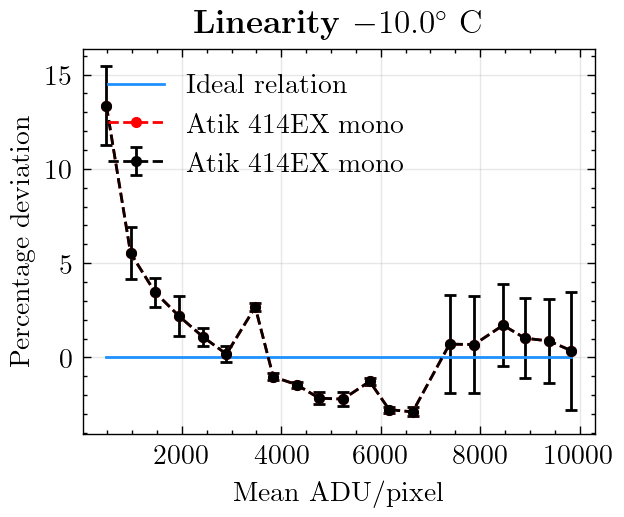
\includegraphics[width=0.6\textwidth]{time_calibration_deviations.png}
		\caption{Linearity deviations are plotted as a function of ADU. These data points are used to compute the first guess of a time correction factor. Data points corresponding to shorter exposure times demonstrate greater deviations, as expected. Larger uncertainties in some of the data points, in particular the first few data points, may be due to instabilities in the light source. }
		\label{fig:timecaldev}
	\end{figure}
		
		\subsection{Linearity}
		The nonlinearity, defined by equation \ref{eq:fluxcorrect_timecal}, for data acquired in exposure times according to section \ref{sec:explin}, may be seen in figure \ref{fig:linearity}. 
		
		Linear behavior is shown with a blue line. The first data point exhibits significant deviation likely due to lack of a proper time calibration. Whether the sixth datapoint is a statistical outlier, or a true peculiarity of the nonlinearity curve, should be determined by a repeat of the experiment. It is not observed in the repeat of the experiment for the dimmed light source in figure \ref{fig:linearitydim}. It must hence be a systematic error in the measurement series. Fluctuations are observed in the low-ADU regime. This corresponds to short exposure times. The fluctuations are seen in the interval between 1 seconds to 10 seconds. The latter point is used as the reference exposure, which is why it correctly displays zero deviation. 
		
		\begin{figure}
			\centering			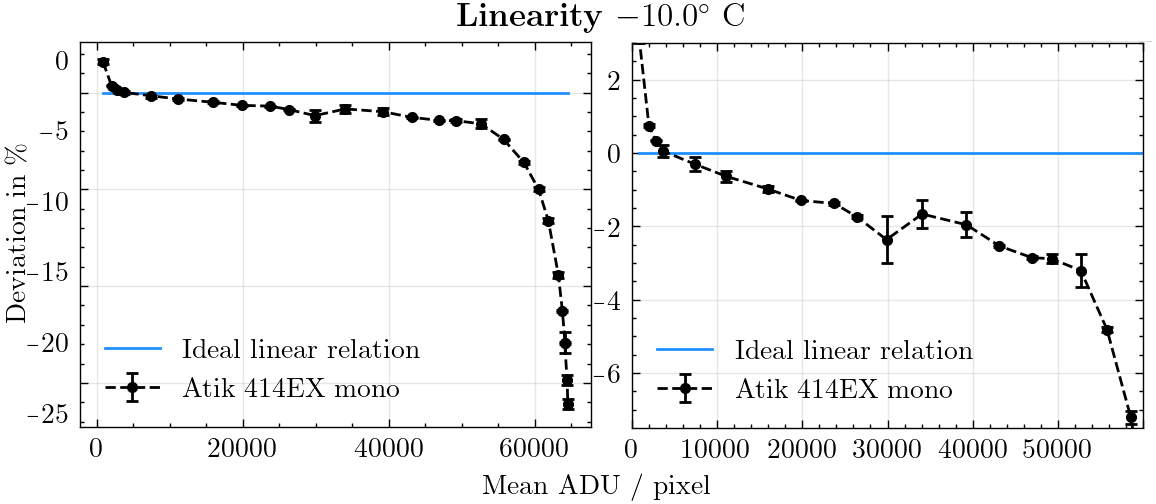
\includegraphics[width=0.999\textwidth]{linearity_timecorrect_final.png}
			\caption{A plot of the percentage deviation from linearity, computed from equation \ref{eq:fluxcorrect_timecal}. Here the time calibration has been applied. Left: The nonlinearity curve as in figure \ref{fig:linearity}, but with the time calibration applied. A dimmed light source of roughly half the intensity was used. Right: Zoom of the left pane. Cf. figure \ref{fig:linearity} (no time calibration, no dimming) the data points seem to be better correlated. The deviation observed is of the same order of magnitude, but appears much better correlated between adjacent points. }
			\label{fig:linearitydim}
		\end{figure}
		
		Figure \ref{fig:linearitydim} is a new data set, with the time calibration applied and using a dimmer light source. Here the time calibration, which is measured and tabulated in \ref{table:results}, is applied. Dimming was achieved by turning off 'half' of the flourescent light bulbs in the room, resulting in roughly half the intensity of light. 
		For this dimmed light setting, low ADUs correspond to longer exposure times, and the time offset is of lesser importance, since it corresponds to a much smaller fraction of the total exposure time. It is in fact seen, that the curve remains the same with or without the time calibration. This is however not the case for \ref{fig:linearity}, where the time calibration is more important due to the shorter exposure times. For this data set the exposure times in
		$[5, 10, 20, 30, \dots 230, 240]$, all in units of seconds, have been used. 
		
		The first data points exhibit the same order of magnitude of deviation, but the deviation is now correlated between adjacent points. This indicates that we have found the true nonlinearity of the detector.
		
		In order to test our estimate of the time offset from equation \ref{eq:timecalprec}, we may fit a linear curve to the data in figure \ref{fig:linearitydim}, giving us an estimate of the \textit{true} linearity at the faulty points. This can be used to correct the fluxes in equation \ref{eq:timecalprec}, and yields a new time offset. We can reinsert this in our analysis, and this process may be iterated until convergence. This was attempted, but with no significant improvement in the deviations. This is also evidence that we have obtained the true linearity curve. In addition we can conclude that we have found the proper time calibration in equation \ref{eq:timecalprec}.
		
		This is considered the final desired linearity curve. The data is tabulated for the Atik 414EX detector in table \ref{table:linearitydata}. This data may be used to calibrate the detector.
		
		%The error is reduced by choosing a dimmer light source. Qualitatively the nonlinearity curve looks very similar, as it should, since in the ADU space we are independent of exposure times. Finally, in order to verify that dimming improves the response in the low-ADU regime, we can attempt to dim the light even more. This was done in \ref{fig:linearitydim}, where a smaller flourescent light bulb was used. Deviations in the low ADU regime is significantly smaller. A few data points in the middle of the dynamic range were omitted due to a systematic error. 
		It is recommended that \textbf{the entire linearity curve is acquired at a dim light setting}, such that the low-ADU regime does not correspond to short exposure times, and the time calibration is of lesser importance. 
		%\begin{figure}
		%	\centering			%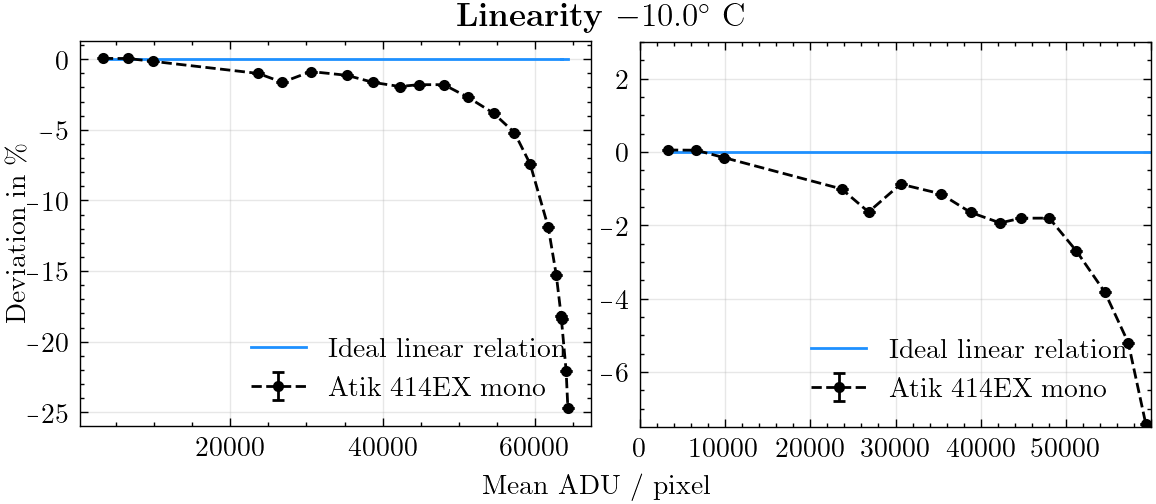
\includegraphics[width=0.999\textwidth]{linearity_dimmed_final.png}
		%	\caption{Left: A plot of the percentage deviation from ideal linearity, computed from equation \ref{eq:fluxcorrect_timecal}. Here the data is using an even dimmer light source, in order to decouple the low ADU regime from a low exposure time regime, such that the time offset becomes of lesser importance. A few datapoints had to be omitted due to a systematic error. Right: a zoom of the left pane.}
		%	\label{fig:linearitydim}
		%\end{figure}
	%\begin{figure}
	%	\centering			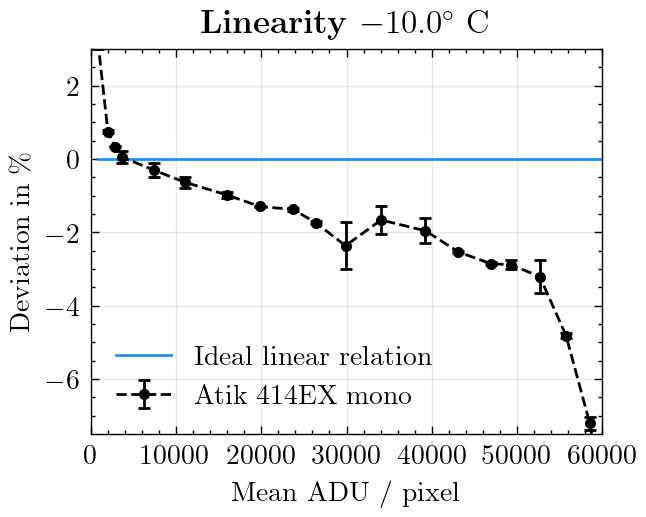
\includegraphics[width=0.7\textwidth]{linearity_zoom_atikcam_dimmed.png}
	%	\caption{A zoom in of figure \ref{fig:linearitydim}. A plot of the percentage deviation from ideal linearity, computed from equation \ref{eq:fluxcorrect_timecal}, with a dimmed lightsource of roughly half the intensity.}
	%	\label{fig:linearitydimzoom}
	%\end{figure}
		
		
		\subsection{Digital saturation}\label{sect:digsat}
		Saturation of the detector pixels is one of two things: Either we have reached the full well of a pixel, or the charge value, once read out and digitized, is greater than what is representable with the number of available bits in the ADC. The first phenomenon is a physical saturation, and the latter is a digital saturation. Consider figure \ref{fig:linearitydim}. There is a significant drop-off around $60000$ ADU, and the curve looks asymptotic around a value just above $65000$ ADU. We wish to determine whether this behavior is due to digital saturation. 
		
		Ideally, the detector is designed such that a full well corresponds to an ADU value below digital saturation. When a pixel reaches full well, the charge will start to 'spill' into neighboring pixels via diffusion processes. We call this effect \textbf{bleeding}. The curve in figure \ref{fig:linearitydim} is the mean behavior of the pixels. If the functional behavior of the curve is due to physical saturation, we should expect to observe that all pixels are saturated. This occurs due to filling by incoming photons, or electrons bleeding over from neighboring pixels. This effect is gradual with increasing exposure times. For true saturation, an arbitrarily chosen single pixel should exhibit a gradual fall-off asymptotically toward some ADU value corresponding to full well. 
		
		The ADC of the Atik 414EX detector, has a 16-bit architecture. The maximum value we may represent with 16 bits is an ADU value of $65536$. Consider figure \ref{fig:linearitydim}. If we study the linearity curve of an arbitrarily chosen single pixel and notice a sudden discontinuous drop-off, we must identify the effect as digital saturation. 
		
		The linearity curve of a single arbitrarily chosen pixel is plotted in figure \ref{fig:linearitydimonepix}. We notice a sudden drop-off of the curve, corresponding to the maximum representable value of $16$ bit. We may thus conclude that our detector has issues with digital saturation, and we should ensure that we do not acquire exposures close to this ADU value.
		
		\begin{figure}[h!]
			\centering			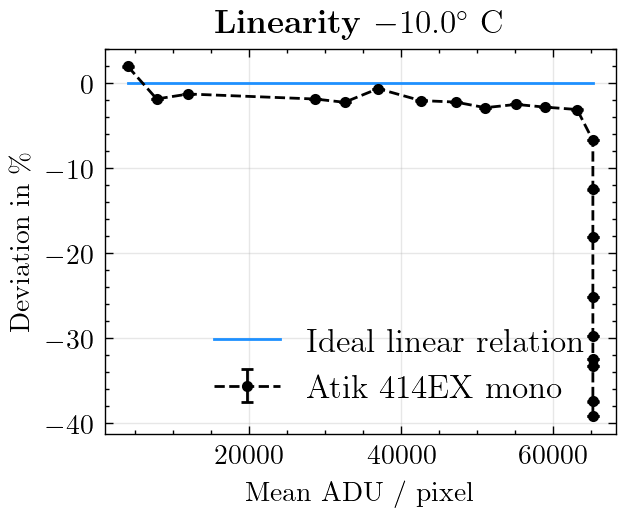
\includegraphics[width=0.7\textwidth]{linearity_onepixel.png}
			\caption{The linearity curve for an arbitrarily chosen single pixel. We observe digital saturation, as described in section \ref{sect:digsat}. There were errors in the measurement sequence of the $40s, 50s$ and $60s$ exposures. These data points were omitted in the analysis. This was due to all of the lights having been turned on in the room by accident, during the acquisition of those data points.}
			\label{fig:linearitydimonepix}
		\end{figure}
		
		\clearpage
		\section{Measurement plan} \label{sec:charmeasplan}
		This chapter will present and describe the test procedure measurement plan that results from the conclusions drawn in the preceding chapter. It will be presented in the most general sense as a step by step guide to obtaining the data. The setup assumed is that seen in figure \ref{fig:setup}.
		
		The first crucial steps is to get a sense of the dynamic exposure range of the camera before proceeding. A few frames should be acquired to study the saturation of the camera. Saturation was observed at an exposure time of about $240$ seconds for the test procedure camera using the dimmed light setting. Thus the ADU range of interest is $[0.001s, 240s]$.
		
		\subsection{Preparations and corrections}
		\begin{enumerate}
			\item \textbf{Temperature setpoint:} If the detector has a cooling system, set the temperature low. This ensures that signal to noise levels are improved. This temperature setpoint should be held constant throughout the characterization procedure. For the Atik 414EX detector this was $-10^\circ$ degrees.
			\item \textbf{Master bias frame:} In a dark room, acquire $N=300$ repeat frames with the detectors' minimal exposure time. For the Atik 414EX detector, this exposure time was $0.001s$. Mean over the images to construct the master bias frame.
			\item \textbf{Master flat-field frame:} In a lit room acquire $N=300$ repeat frames of the white screen at an exposure time in which any contrast from the non-flatness is seen properly. For the Atik 414EX detector, a $10s$ exposure time was chosen. Mean over the frames to construct the master flat-field frame.
			\item \textbf{Readout noise level:} At the chosen temperature, compute the readout noise level as described in section \ref{ron}, using the bias frame series acquired above. This yields the readout noise level in ADUs. For the Atik 414EX detector this was $13.044$ RMS ADU.
			\item \textbf{Gain measurement:} Use two flat-field frames acquired in the data series of flat-field frames acquired above to compute the gain factor as in equation \ref{eq:gainfactorest}. Do this using the rest of the data series to improve precision, by meaning over the gain factors obtained. For the Atik 414EX detector this was computed to be $0.24$  electrons/ADU for $-10^\circ$, while the tabulated value \cite{atik414specs} was  $0.28$  electrons/ADU.
			\item \textbf{Time calibration:} 
			At three different light source intensities (flux levels), acquire  $N=10$ repeats of the series $\bm F_1[s]_\text{before} \rightarrow \bm F_2[s] \rightarrow \bm F_1[s]_\text{after}$. The exposure times should correspond to the low end of the ADU range. For the Atik 414EX detector this was two $1\text{s}$ measurement sandwiching a $2\text{s}$ measurement. For each repeat, compute the time offset from equation \ref{eq:timecorrectionfactor} and mean over the $N$ repeats. Do the same for the other two flux levels, and mean over these $3$ values. This yields the time correction uncoupled from light source intensity and statistical fluctuations.
			%$[0.5s, 1s, 1.5s, \dots, 9s, 9.5s, 10s]$.
			%\begin{itemize}
			%	\item At each exposure time, acquire $N = 10$ repeats that will be meaned over.
			%	\item For each datapoint acquire a $10s$ reference measurement before and after, to correct for lightsource instability as according to the description outlined above
			%	\item For each exposure time construct a mean image from repeats
			%	\item For each of these mean images, one at every exposure time, and the reference measurements respectively before and after:
			%	\begin{itemize}
			%		\item Subtract master bias frame from each of the three images.
			%		\item Set hot pixels equal to mean value of the image, where hot pixels are omitted.
			%		\item Compute the mean ADU/pixel in each image
			%		\item Fit a linear relation to the data
			%		\item Find the roots of the polynomium, which will be interpreted as the temporal offset due to the lack of a shutter
			%	\end{itemize}
			%\end{itemize}
		\end{enumerate}
		
		\subsection{Linearity}
		\begin{enumerate}
			\item Acquire frames while varying exposure times, covering the entire ADU range. At a given flux level (held a constant throughout the measurement series acquisition), acquire an image at an exposure for which the frame begins saturating visibly. This exposure time will be the end of the range. For the test procedure camera, at the flux level corresponding to half the light bulbs turned on, this was an exposure time of $240s$. 
			
			Choose an exposure time that serves as a reference exposure, which for the test procedure camera, was chosen arbitrarily to be $10$s. 
			
			Acquire evenly spaced frames at varying exposures in this ADU range. For the test procedure camera this was the exposure times
			$[10, 20, \dots 230, 240]$, all in units of seconds.
			\begin{itemize}
				\item At each exposure time, acquire $N = 10$ repeats that will be meaned over.
				\item For each datapoint acquire a reference measurement before and after, to correct for lightsource instability as according to the description outlined above in section \ref{sec:linearity}.
			\end{itemize}
			\item For each exposure time construct a mean image from repeats.
			\item For each of these mean images, and the reference images taken before and after:
			\begin{itemize}
				\item Subtract the master bias frame from each of the three images.
				\item Set hot pixels equal to mean value of the image (the mean calculated, not including the hot pixels themselves).
				\item Compute the mean ADU/pixel in each image.
				\item Compute the nonlinearity according to equation \ref{eq:fluxcorrect_timecal}.
			\end{itemize}
		\end{enumerate}
		
		This produces a plot like figure \ref{fig:linearitydim}.
		
		\subsection{Temperature dependence of noise}\label{sec:rondc}
		 If the camera has cooling capabilities, we should sample the entire cooling temperature range evenly. For the Atik 414EX detector, the series [-10, -8,$\dots$ 20] (in $^\circ$ deg.). For each temperature acquire
			\begin{itemize}
				\item $100$ bias frames at the minimal exposure time as described above. For the test procedure detector this was an exposure time of $0.001$s. These frames are used to compute the readout noise as a function of temperature
				\begin{itemize}
					\item At every temperature consider each repeat image in turn. Compute the mean ADU/pixel and subtract it from every pixel in the image. The resulting image is a stochastic Gaussian distribution with a mean of zero
					\item Multiply every pixel with the camera gain converting ADUs to electrons.
					\item Compute the standard deviation of the flattened array of pixels.
					\item This yields $100$ standard deviations, and from this, a RMS value is computed. These values can then be plotted as a function of temperature.
				\end{itemize} 
				\item $100$ dark frames at $10.0s$ exposure time
				\begin{itemize}
					\item For each temperature sequence, construct a mean image to improve the signal to noise ratio in the image.
					\item Subtract the master bias frame.
					\item Set hot pixels equal to mean value of the image, where hot pixels are omitted.
					\item Multiply every pixel with the camera gain, to convert ADUs to electrons.
					\item Divide every pixel with the exposure time.
					\item Compute mean ADU/pixel.
				\end{itemize}
			\end{itemize}
		The result of these two analyses may be seen plotted in figures \ref{fig:readoutnoise} and \ref{fig:darkcurrent}.
		
		
		\section{Proof of concept: Characterizing the Prosilica GC660M camera}\label{sec:avtchar}
		In order to give proof of concept, and verify the characterization procedure, the procedure should be applied to a different detector. This was done for a \textbf{AVT Prosilica GC660M} camera. A picture of the camera is seen in figure \ref{fig:avtcam}. The specs for the camera have been tabulated in table \ref{table:avtcam}. In comparison to the Atik 414EX detector, this camera houses a Sony ICX 618 sensor, which is a progressive scan CCD like the Atik 414EX detector. In addition the camera has an adjustable aperture that enables the user to more or less control the amount of incoming light. It also has an adjustable mounted lens. 
		
		\begin{figure}[hbt!]
			\centering			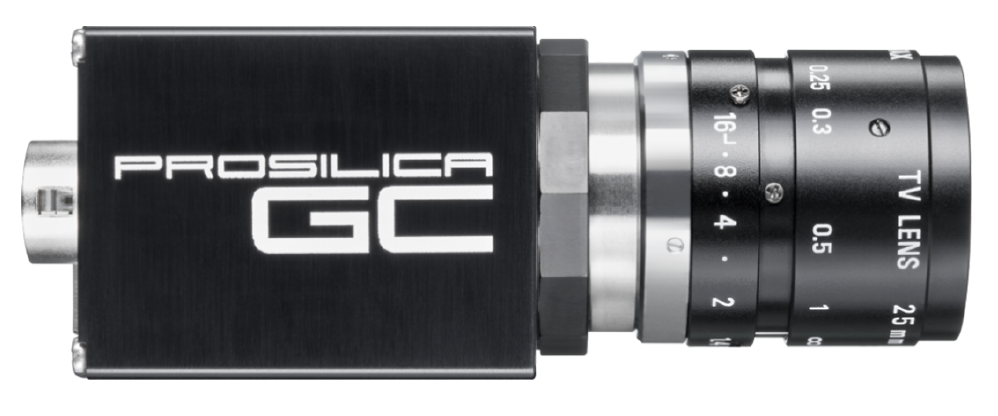
\includegraphics[width=0.5\textwidth]{prosilica_gc660M.png}
			\caption{A picture \cite{avtcamspecs} of the AVT Prosilica GC 660M camera that was used to verify the characterization procedure. The camera consists of a Sony ICX 618 sensor, which is a progressive scan CCD like the Atik 414EX detector. The camera has a mounted lens and an aperture that is adjustable, letting in more or less light. The camera does not have cooling capabilities.}
			\label{fig:avtcam}
		\end{figure}
		
		\subsection{Initial considerations}
		The same experimental setup was used (cf. figure \ref{fig:setup}). The adjustable lens was focused at the white screen. No pinhole was made for this camera, due to the aperture and lens enabling greater control of the amount of incoming light, and focusing of the image. The aperture was set to the minimal radius setting, to block as much incoming light as possible.
		
		\subsection{Running the test procedure}
		According to the measurement plan, a bias frame was constructed in a dark room from $N=300$ repeats of an exposure time of $0.001s$. This frame may be seen in figure \ref{fig:avtbias}.
		
		The camera at hand does not have a cooler, so the remainder of the measurement plan consists of acquiring frames in a lit room setting. The same light source was used. The light source was dimmed as described above. We need to get a sense of the dynamic range of the camera before we can proceed, so a few frames were acquired to study the saturation of the camera. Saturation was observed at an exposure time of about $4$ seconds. Thus when performing linearity measurements, this exposure time is likely to be at the end of the ADU range, and measurements should be performed in the interval $(0s, 4s]$. The exposure time for the flat-field was chosen to be $1s$.
		
		\begin{figure}
			\centering			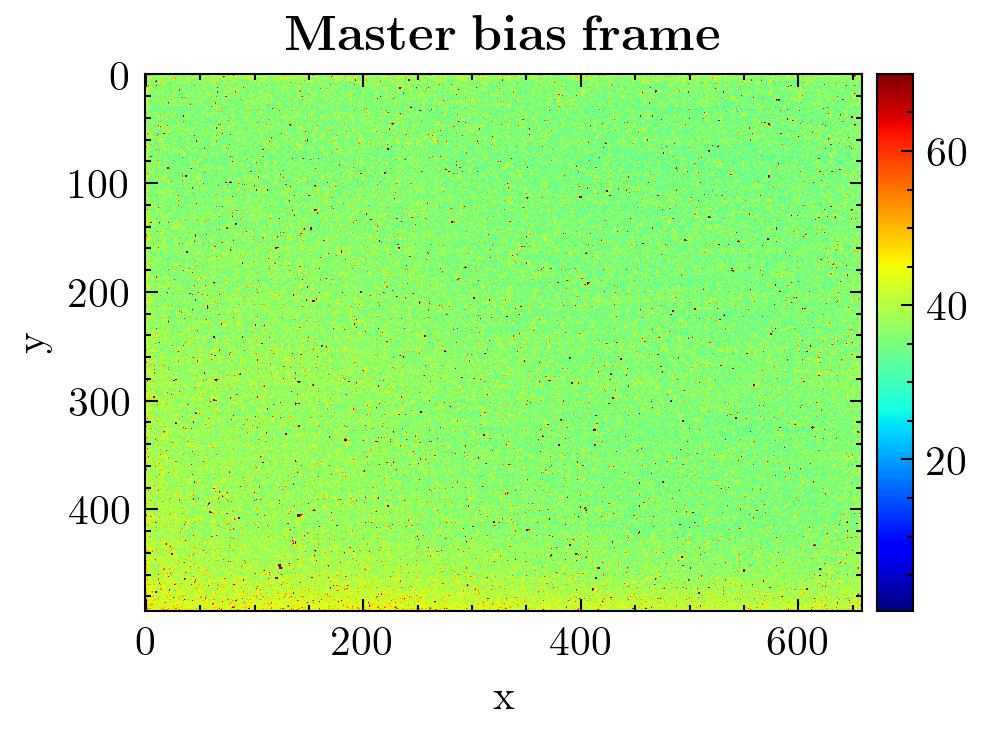
\includegraphics[width=0.65\textwidth]{master_bias_AVT.png}
			\caption{The master bias frame for the AVT camera. The bias frame of the AVT camera shows a flat chip structure, but significant noise contributions and some hot pixels when comparing to the bias frame of the Atik camera used in development of the testing procedure (cf. figure \ref{fig:masterbias}).}
			\label{fig:avtbias}
		\end{figure}
		
		A master flat-field was then constructed using $N=300$ repeats of images of a white screen taken at an exposure time of $1s$. This frame can be seen in figure \ref{fig:avtflat}. 
	
		\begin{figure}[hbt!]
			\centering			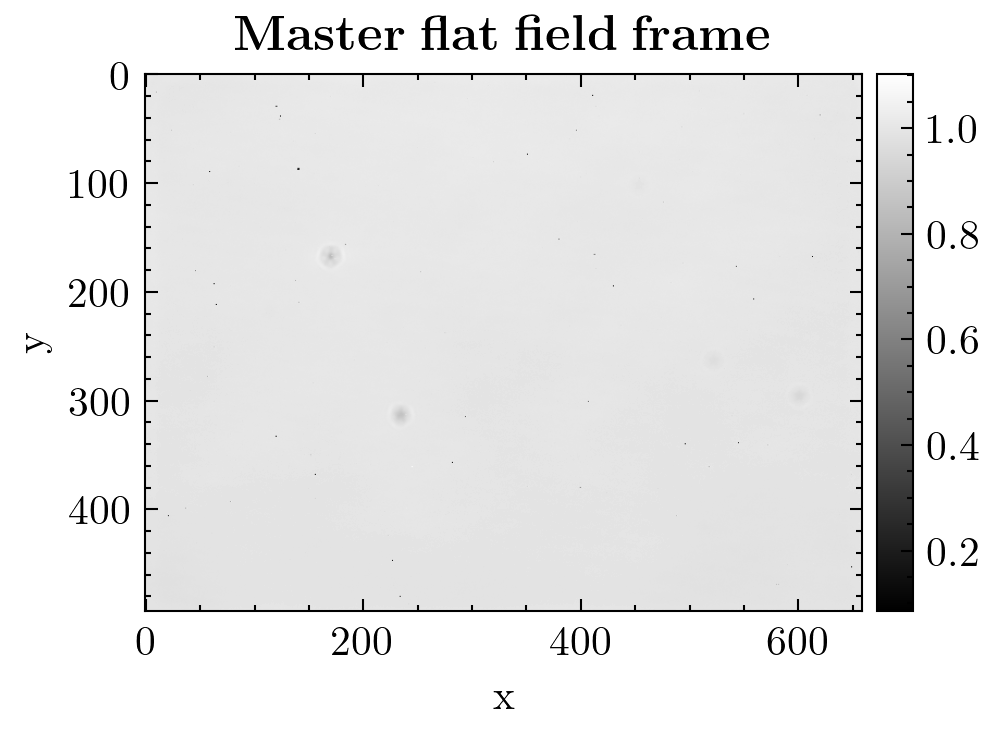
\includegraphics[width=0.8\textwidth]{master_flat_AVT.png}
			\caption{The master flat-field frame for the AVT camera. The flat frame of the AVT camera is very flat, with only a few specks of dust visible on the lens.}
			\label{fig:avtflat}
		\end{figure}
	
		This camera does not have a mechanical shutter, and we msut expect a contribution to the exposure time from the time calibration. This is performed using the exposure times $0.1\text{s}_\text{before} \rightarrow 0.2\text{s} \rightarrow 0.1\text{s}_\text{after}$ at the same light source intensities as was used to develop the testing procedure. A time calibration factor of $-0.0094s$ was computed, corresponding to a longer exposure time by $0.009$ seconds. 
		
		\begin{table}[]
			\centering
			\begin{tabular}{|c|c|}
				\hline
				\textbf{Model name }& AVT Prosilica GC660M \\
				\textbf{Chip name}&  Sony ICX 618\\
				\textbf{Readout noise (typical)}& Not specified\\
				\textbf{Gain factor}& Variable\\
				\textbf{Cooling $\Delta T$}& No cooling\\
				\textbf{Dark current}& $\sim 16.7 e^- / s\;$\\
				\textbf{ADC}& 12 bit\\
				\textbf{Pixel size}& $5.6 \mu \text{m} \times 5.6 \mu \text{m}$\\ 
				\textbf{Shutter}&No\\
				\hline
			\end{tabular}
			\caption{Relevant data specs for the \textbf{AVT Prosilica GC 660M} camera \cite{avtcamspecs}. Here a variable gain factor means that it may be set arbitrarily by software available from the manufacturer.}
			\label{table:avtcam}
		\end{table}
		
		Finally, the linearity of the camera was investigated. In intervals of $0.1s$ exposures, images were acquired in the range $[0.1s, 4s]$ using $N=10$ repeats. A $1s$ exposure image, before and after each exposure was used as a reference. The linearity was computed as described above. The result may be seen in figure \ref{fig:avtlinearity} serves as a proof of concept for the testing procedure. Nonlinearity in the same order of magnitude as that for the Atik 414EX detector is found, with sampled data points distributed evenly and well-correlated within the entire dynamic range of the camera. A digital saturation is observed at an ADU value of $4096$ corresponding to the maximum value that can be represented by the $12$ bit ADC. 
		
		\begin{figure}[hbt!]
			\centering			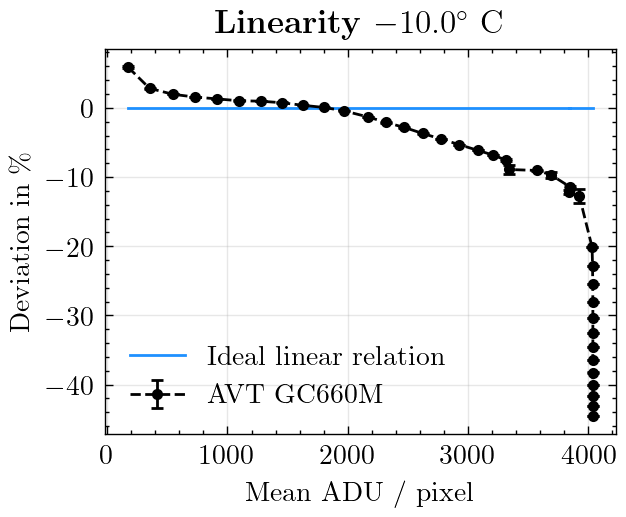
\includegraphics[width=0.7\textwidth]{linearity_AVT.png}
			\caption{The linearity curve for the AVT camera, computed as specified in the measurement plan. The nonlinearity is in the same order of magnitude as for the test procedure camera, and the data points are observed to be well correlated and evenly distributed within the dynamic range of the camera. We observe positive deviations in the start of the curve, due to the time calibration, as was the case for the Atik 414 EX detector. In addition, digital saturation is observed, as for the Atik 414EX detector, since a significant saturation effect is observed around the ADU value of $12$ bits $=  2^{12}$ ADU$ = 4096$ ADU. The dip observed around $3300$ ADU, and the one at 3800 ADU (two datapoints lie on almost on top of one another) appears to be an artifacts of the true linearity, as they were reproduced in a subsequent measurement. These may be due to the amplification stage electronics.}
			\label{fig:avtlinearity}
		\end{figure}
	
	\section{Results and requirements from scientific requirements}\label{sec:firstreq}
	A summary of the obtained results from the characterization procedure, along with computed errors, may be found tabulated in table \ref{table:results}. There are a few discrepancies between tabulated and measured results. 
	
	For the Atik 414EX detector, the dark current is measured to be an order of magnitude greater than the tabulated value. Pixels may go bad with time, for example due to radiation damage from cosmic rays or high energy particles, and this may be part of the explanation for this discrepancy.
	Readout noise is measured to be lower, but the manufacturer had not specified a temperature for which the value was tabulated, which is the most obvious explanation for the difference observed. The gain factor is measured to be slightly lower than the tabulated value, but is of same order of magnitude. This difference is not likely due to temperature differences, as is evident from figure \ref{fig:gainvtemp}, but is more likely due to changes in the amplifications or digitization stage of the detector.
	
	For the AVT Prosilica GC660M camera, most of the values had not been specified by the manufacturer, so a comparison is moot.
	\begin{table}[]
		\centering
		\begin{tabular}{|
				>{\columncolor[HTML]{C0C0C0}}l ll|}
			\hline
			\multicolumn{3}{|c|}{\cellcolor[HTML]{C0C0C0}{\color[HTML]{000000} \textbf{\begin{tabular}[c]{@{}c@{}}Characterization results\\ Temp: $-10^\circ$\end{tabular}}}}                                                             \\ \hline\hline
			\multicolumn{3}{|c|}{\cellcolor[HTML]{C0C0C0}{\color[HTML]{000000} \textbf{ATIK 414EX mono}}}                                                                                                                                                  \\
			{\color[HTML]{000000} }                                                                                                   & \cellcolor[HTML]{C0C0C0}{\color[HTML]{000000} Tabulated} & \cellcolor[HTML]{C0C0C0}{\color[HTML]{000000} Measured} \\ \cline{2-3} 
			\multicolumn{1}{|l|}{\cellcolor[HTML]{C0C0C0}{\color[HTML]{000000} \textbf{Dark current}}}                                & {\color[HTML]{000000} $\sim 0.001 \;e^-/s$}                & {\color[HTML]{000000} $\sim 0.028 \pm 0.032 e^-/s$}     \\
			\multicolumn{1}{|l|}{\cellcolor[HTML]{C0C0C0}{\color[HTML]{000000} \textbf{Readout noise}}}                               & {\color[HTML]{000000} $5 \;e^-$}                           & {\color[HTML]{000000} $ 3.227 \pm 0.096 $ RMS $e^-$}     \\
			\multicolumn{1}{|l|}{\cellcolor[HTML]{C0C0C0}{\color[HTML]{000000} \textbf{Gain factor}}}                                 & {\color[HTML]{000000} $0.28 \;e^-/$ADU}                    & {\color[HTML]{000000} $0.24384  \pm  0.00005 \; e^-/$ADU}   \\
			\multicolumn{1}{|l|}{\cellcolor[HTML]{C0C0C0}\textbf{\begin{tabular}[c]{@{}l@{}}Time calibration \\ factor\end{tabular}}} & N/A                                                      & $-0.005 \pm 0.003 s$                                    \\ \hline
			\multicolumn{3}{|c|}{\cellcolor[HTML]{C0C0C0}\textbf{AVT Prosilica GC660M}}                                                                                                                                                                    \\
			& \cellcolor[HTML]{C0C0C0}Tabulated                        & \cellcolor[HTML]{C0C0C0}Measured                        \\ \cline{2-3} 
			\multicolumn{1}{|l|}{\cellcolor[HTML]{C0C0C0}\textbf{Dark current}}                                                       & $\sim 16.7 e^-/s$                                        & N/A                                                     \\
			\multicolumn{1}{|l|}{\cellcolor[HTML]{C0C0C0}\textbf{Readout noise}}                                                      & N/A                                                      & $20.276 \pm 0.047 $ RMS $e^-$    \\
			\multicolumn{1}{|l|}{\cellcolor[HTML]{C0C0C0}\textbf{Gain factor}}                                                        & N/A                                                      & $5.323  \pm  0.003 \;e^-/$ADU                             \\
			\multicolumn{1}{|l|}{\cellcolor[HTML]{C0C0C0}\textbf{\begin{tabular}[c]{@{}l@{}}Time calibration \\ factor\end{tabular}}} & N/A                                                      & $-0.009 \pm 0.005 \;s$                                    \\ \hline
		\end{tabular}
	\caption{A summary of the results computed from application of the characterization procedure to both the the Atik 414EX detector, and the AVT Prosilica GC660M camera, compared to those tabulated by the manufacturer in \cite{atik414specs, avtcamspecs}. The temperature was set to $-10^\circ$ for the Atik 414EX detector, and room temperature for the AVT Prosilica GC660M camera (which lacks cooling capabillities). Dark current has been computed as outlined in section \ref{sec:dc}, but not for the AVT Prosilica GC660M camera, as the manufacturer had not specificed a temperature setpoint. The dark current value for the Atik 414EX detector corresponds to the first datapoint in figure \ref{fig:darkcurrent} with its relative error. Readout noise is computed as described in section \ref{ron}, and the gain factor as described in section \ref{sec:gain}, and the time calibration factor as in \ref{sec:timecal}. For the Atik 414EX detector, these values for the readout noise and gain factor, along with corresponding relative errors, correspond to those plotted in figures \ref{fig:ronmeas} and \ref{fig:gainmeasurement}.}
	\label{table:results}
	\end{table}
	
	One of the two mission requirements outlined in the introduction relates to photometric precision. If we consider time-series photometric data of a planetary transit, we observe a dip in the relative flux of the light. The very concept of a transit depth relies on a comparison between two different ADU levels. Therefore the linearity of the detector will be important. The more precisely we have measured the linearity curve, the more precisely we can measure the transit depth. This means we are more certain of the actual size of the planet that we have observed. The mission requirement relating to the photometric precision is required to be $10^{-4}$. The error bars in figure \ref{fig:linearitydim} are in the range of magnitude $10^{-3}-10^{-4}$, or $0.1\% - 0.01\%$. These are also tabulated in table \ref{table:linearitydata}. The linearity curve has been constructed using $N = 10$ repeats of each data point. Since we are dealing with counting statistics (Poissonian statistics), the relative error in the measurement $\sigma / \sqrt{N}$ will decrease by a factor of $\sqrt{M}$ if we increase the number of measurements by a factor of $M$. If we repeat the measurement series $100$ times, this corresponds to increasing the precision by an order of magnitude. 
	
	The first conclusion is that the Atik 414EX detector can reach the desired photometric precision stated in the introduction. A second conclusive remark may be that, if the detector that will be flown on the STEP mission does not meet this requirement using $N = 10$ measurements, we may repeat the measurement of the linearity curve until we reach the desired precision. Each time we repeat the experiment $100$ times we gain an order of magnitude. For some detectors this will be subsequent to requirements trading if this is practically infeasible, perhaps due to time constraints, resulting in choosing a \textit{better suited} detector.
	
	\section{How to apply the results}\label{sect:cal}
	In the preceding sections, the characterization procedure, and the theory it is predicated on, have been explained in detail. The point of the characterization procedure is to be able to calibrate the detector for use in scientific measurements. 
	
	\subsection{Bias and hot pixel corrections}
	After construction of the master bias- and flat-field frames, these are used as corrections in subsequent measurements. The master bias is always subtracted first. Afterward, the hot pixel mask is used to correct for hot pixels. This may be used as a mask of pixels to omit in the data analysis of the signal, or these pixels may be set to the mean ADU value of the image (computed from the image where the hot pixels are omitted), in the remainder of the data analysis. 
	
	\subsection{Gain and nonlinearity}
	The linearity correction is used to calibrate the flux levels in the signal. The nonlinearity curve is a function of ADU, and the image is to be corrected for nonlinearity on a pixel-by-pixel basis. Say for a given ADU value, in a given pixel, the nonlinearity (as seen in figure \ref{fig:linearitydim}) is measured to be $1\%$. In this case, the signal, after the corrections from the preceding section have been applied, is divided by $1.01$. If the nonlinearity was $-1\%$, it is divided by $0.99$ and so on. In general
	\begin{equation}
		\text{ADU}(x,y)_\text{linearity corrected} = \frac{\text{ADU}(x,y)_\text{Bias and hot pixel corrected}}{\delta(\text{ADU}(x,y))}
	\end{equation}
	 Where $\delta(\text{ADU}(x,y))$ is as in equation \ref{eq:fluxcorrect_timecal}. These calibration values are tabulated for the Atik 414EX detector in table \ref{table:linearitydata}.
	 
	 After correcting for the nonlinearity, we may correct for gain, and interpret the signal in electrons. This may also be done after flat field correcting.
	 
	 \subsection{Flat field corrections}
	 Lastly the flat field correction is applied by dividing the image, on a pixel-by-pixel basis, by the master flat field frame. This concept is explained, in detail, in section \ref{sec:flat}. This step is very important in photometric measurements.
	 
 	\newpage
 	\begin{table}[]
 		\centering
 		\begin{tabular}{|l|l|l|}
 			\hline
 			\rowcolor[HTML]{C0C0C0} 
 			{\color[HTML]{000000} \textbf{Exposure time {[}s{]}}} & {\color[HTML]{000000} \textbf{ADU value}} & {\color[HTML]{000000} \textbf{$\delta(\text{ADU})$ (Linearity) {[}\%{]}}} \\ \hline
 			2                                                     & 822                                 & $3.22 \pm 0.23$                                    \\ \hline
 			5                                                     & 2012                                & $0.73 \pm 0.04$                                    \\ \hline
 			7                                                     & 2805                                & $0.34 \pm 0.01$                                    \\ \hline
 			10                                                    & 3707                                & $0.05 \pm 0.16$                                    \\ \hline
 			20                                                    & 7389                                & $-0.31 \pm 0.20$                                   \\ \hline
 			30                                                    & 11070                               & $-0.64 \pm 0.14$                                   \\ \hline
 			40                                                    & 15922                               & $-0.98 \pm 0.08$                                   \\ \hline
 			50                                                    & 19841                               & $-1.29 \pm 0.02$                                   \\ \hline
 			60                                                    & 23756                               & $-1.38 \pm 0.05$                                   \\ \hline
 			70                                                    & 26373                               & $-1.74 \pm 0.04$                                   \\ \hline
 			80                                                    & 29879                               & $-2.37\pm 0.63$                                    \\ \hline
 			90                                                    & 34052                               & $-1.67 \pm 0.38$                                   \\ \hline
 			100                                                   & 39257                               & $-1.96 \pm 0.35$                                   \\ \hline
 			110                                                   & 43129                               & $-2.53 \pm 0.02$                                   \\ \hline
 			120                                                   & 46947                               & $-2.86 \pm 0.05$                                   \\ \hline
 			130                                                   & 49234                               & $-2.88 \pm 0.12$                                   \\ \hline
 			140                                                   & 52671                               & $-3.21 \pm 0.45$                                   \\ \hline
 			150                                                   & 55742                               & $-4.82 \pm 0.07$                                   \\ \hline
 			160                                                   & 58592                               & $-7.21 \pm 0.18$                                   \\ \hline
 			170                                                   & 60533                               & $-9.96 \pm 0.24$                                   \\ \hline
 			180                                                   & 61880                               & $-13.22 \pm 0.28$                                  \\ \hline
 			190                                                   & 63253                               & $-18.81\pm 0.30$                                   \\ \hline
 			200                                                   & 63812                               & $-22.59 \pm 0.09$                                  \\ \hline
 			210                                                   & 64164                               & $-25.87 \pm 0.09$                                  \\ \hline
 			220                                                   & 64129                               & $-25.84 \pm 1.05$                                  \\ \hline
 			230                                                   & 64449                               & $-29.71 \pm 0.48$                                  \\ \hline
 			240                                                   & 64560                               & $-32.22 \pm 0.53$                                  \\ \hline
 		\end{tabular}
 		\caption{Data acquired for the final linearity curve. Here $\delta(\text{ADU})$ is as in equation \ref{eq:fluxcorrect_timecal}.}
 		\label{table:linearitydata}
 	\end{table}	
\end{document}